\chapter{METODOLOGÍA DE LA INVESTIGACIÓN}
\section{Diseño de la investigación}
En esta sección del documento se explicará cual es el diseño, el tipo y el enfoque del trabajo de
investigación, así como también la población y la muestra. 
%Para finalizar se explicará el
%proceso de aplicación de las redes neuronales convolucionales.
\subsection{Diseño no experimental}
El diseño es no experimental transversal, ya que las variables no serán manipuladas y serán analizadas tal como se encuentran. Es decir, tanto los datos visuales de las hojas de papa peruana afectadas por la enfermedad 'Rancha' (Phytophthora infestans) como las técnicas de visión computacional serán utilizados sin modificar ningún aspecto de las condiciones naturales. El objetivo es aplicar técnicas de visión computacional para clasificar tempranamente la presencia de la enfermedad en las hojas de papa. La recolección de datos se llevará a cabo en un periodo de tiempo específico, sin intervenir en el desarrollo natural de la enfermedad en las plantas

\subsection{Tipo explicativo}
El alcance de esta investigación es explicativo, ya que se enfoca en construir un modelo de visión computacional para la detección temprana de la enfermedad 'Rancha' (Phytophthora infestans) a partir de imágenes de hojas de papa. Esto busca entender cómo identificar si una hoja de papa está afectada por el tizón tardío, estableciendo así una relación de causa y efecto. En otras palabras, al identificar un patrón específico en las hojas de papa con Rancha, se podrá determinar si están afectadas por la patología.

\subsection{Enfoque cuantitativo}
El enfoque de esta investigación es cuantitativo, dado que se emplearán técnicas de visión computacional, las cuales implican procesar datos de imagen en valores numéricos (vectores de características). Posteriormente, se usarán técnicas estadísticas para analizar estos datos y determinar la presencia de la enfermedad 'Rancha' (Phytophthora infestans) en las hojas de papa peruana.

\section{Población }
La población fueron todas las imágenes de hojas de papa infestadas con Tizón tardío hojas de papa sanas. 

\section{Muestra}
La muestra se extrajo un conjunto de imágenes de los dataset Plant Diseases Training Dataset, el cual es una recopilación de otras agrupaciones de datos como PlantVillage, Potato Leaf Disease, Cassava Leaf Disease Dataset, etc. Se cuenta con 1777 imágenes de hojas de papa etiquetadas como sanas y 2020 como infestada con Tizón tardío. Adicionalmente, cabe mencionar, que para el propósito de esta investigación se utilizará 80\% del conjunto de imágenes total para Training y 20\% para el Testing de los modelos correspondientes. La Figura \ref{fig1} y el Cuadro \ref{tab:widgets}

\begin{figure}[h]
	\begin{center}
		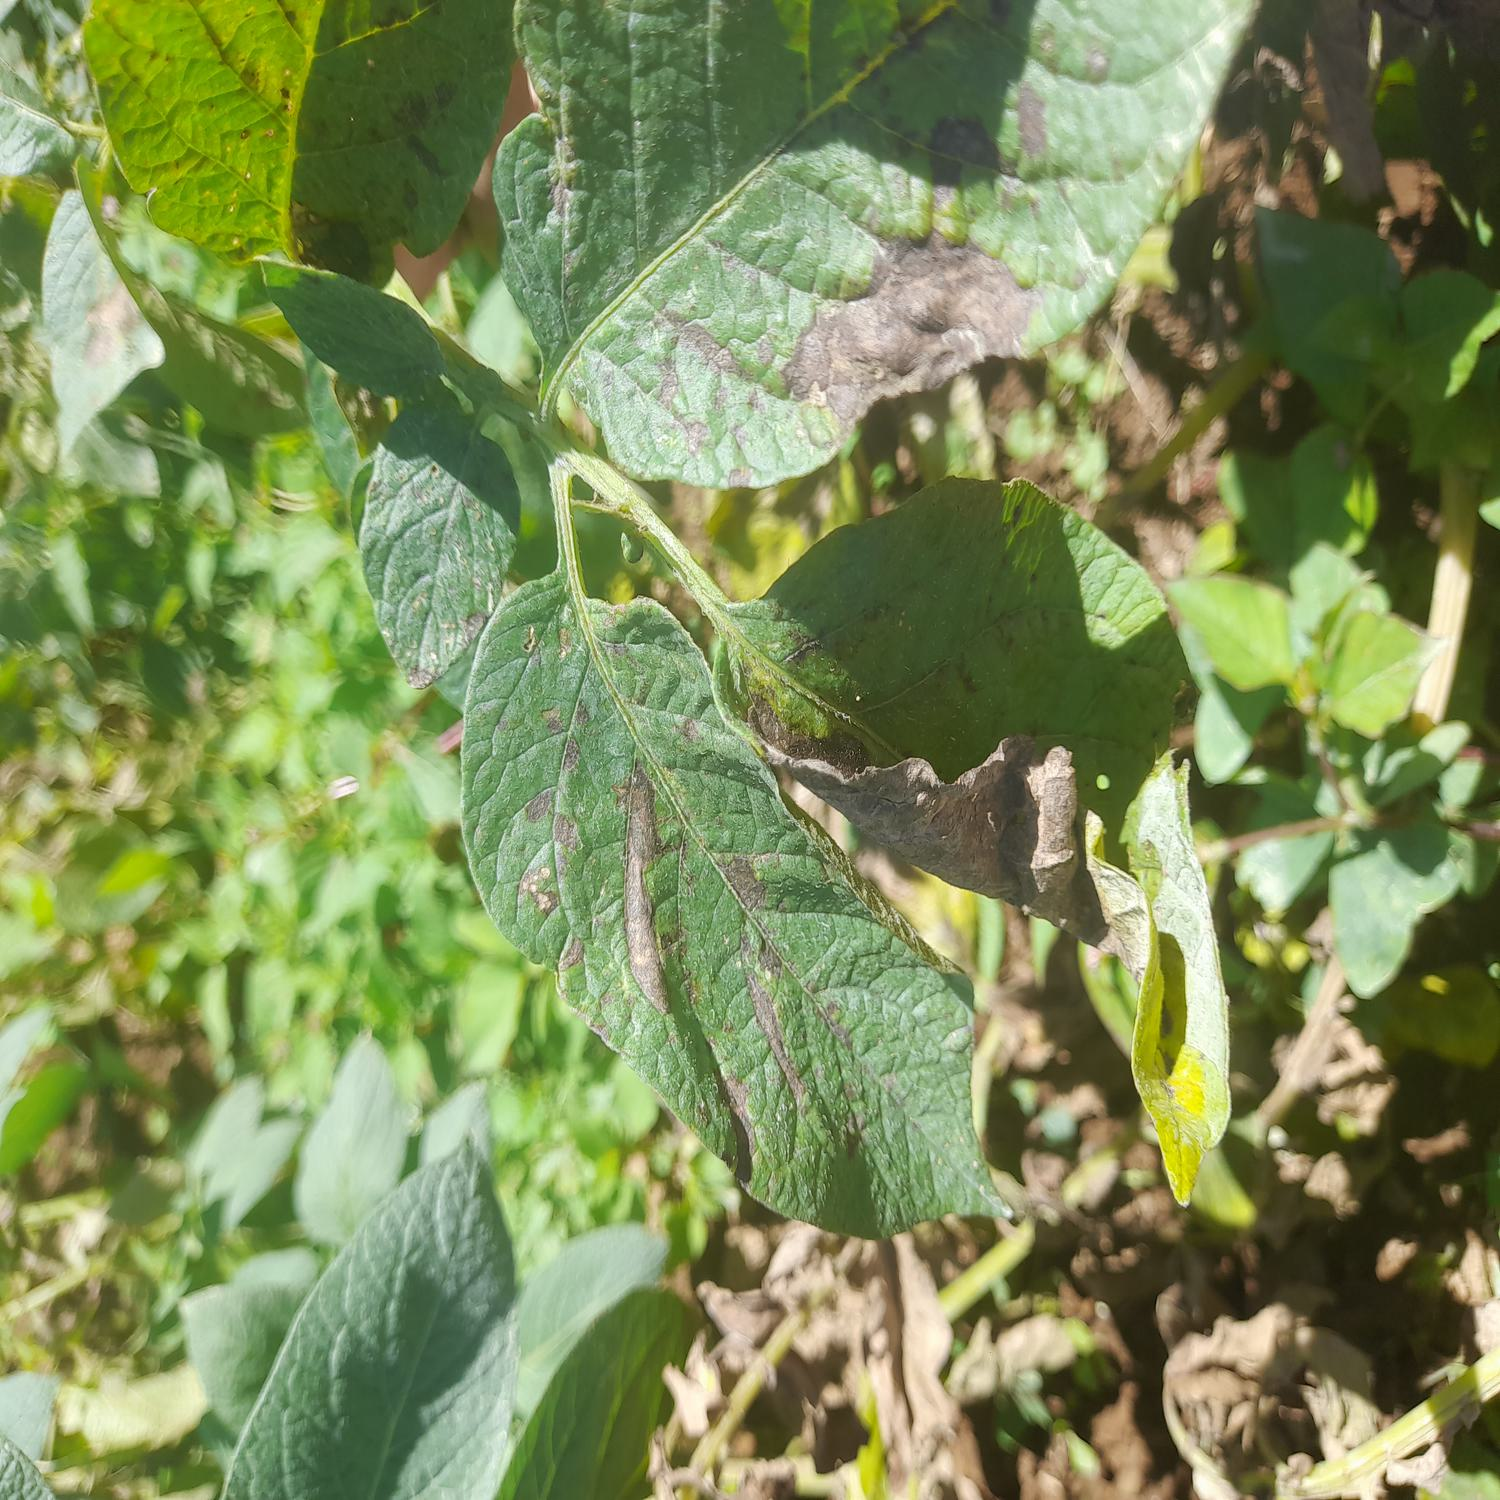
\includegraphics[width=0.8\textwidth]{3/figures/img.jpg}
		\caption{Hoja de papa infestada con Tizón tardío}
		\label{fig1}
	\end{center}
	
\end{figure}

\section{Operacionalización de Variables}

Nisi porta lorem mollis aliquam ut porttitor leo. Aenean pharetra magna ac placerat vestibulum. Est placerat in egestas erat imperdiet sed euismod. Velit euismod in pellentesque massa placerat. Enim praesent elementum facilisis leo vel fringilla. Ante in nibh mauris cursus mattis molestie a iaculis. Erat pellentesque adipiscing commodo elit at imperdiet dui accumsan sit. Porttitor lacus luctus accumsan tortor posuere ac ut. Tortor at auctor urna nunc id. A iaculis at erat pellentesque adipiscing commodo elit.
\section{Instrumentos de medida}
Nisi porta lorem mollis aliquam ut porttitor leo. Aenean pharetra magna ac placerat \begin{itemize}
	\item muscle and fat cells remove glucose from the blood,
	\item cells breakdown glucose via glycolysis and the citrate cycle, storing its energy in the form of ATP,
	\item liver and muscle store glucose as glycogen as a short-term energy reserve,
	\item adipose tissue stores glucose as fat for long-term energy reserve, and
	\item cells use glucose for protein synthesis.
\end{itemize}

\section{Técnicas de recolección de datos}
Nisi porta lorem mollis aliquam ut porttitor leo. Aenean pharetra magna ac placerat vestibulum. Est placerat in egestas erat imperdiet sed euismod. Velit euismod in pellentesque massa placerat. Enim praesent elementum facilisis leo vel fringilla. Ante in nibh mauris cursus mattis molestie a iaculis. Erat pellentesque adipiscing commodo elit at imperdiet dui accumsan sit. Porttitor lacus luctus accumsan tortor posuere ac ut. Tortor at auctor urna nunc id. A iaculis at erat pellentesque adipiscing commodo elit.

\LaTeX{} is great at typesetting mathematics. Let $X_1, X_2, \ldots, X_n$ be a sequence of independent and identically distributed random variables with
\begin{equation}
	S_n = \frac{X_1 + X_2 + \cdots + X_n}{n}
	= \frac{1}{n}\sum_{i}^{n} X_i
	\label{eq1}
\end{equation}

La Ecuación \ref{eq1} denote their mean. Then as $n$ approaches infinity, the random variables $$\sqrt{n}(S_n - \mu)$$ converge in distribution to a normal $\mathcal{N}(0, \sigma^2)$.

\section{Técnicas para el procesamiento y análisis de la información}
Nisi porta lorem mollis aliquam ut porttitor leo. Aenean pharetra magna ac placerat vestibulum. Est placerat in egestas erat imperdiet sed euismod. Velit euismod in pellentesque massa placerat. Enim praesent elementum facilisis leo vel fringilla. Ante in nibh mauris cursus mattis molestie a iaculis. Erat pellentesque adipiscing commodo elit at imperdiet dui accumsan sit. Porttitor lacus luctus accumsan tortor posuere ac ut. Tortor at auctor urna nunc id. A iaculis at erat pellentesque adipiscing commodo elit.

You can make lists with automatic numbering \dots

\begin{enumerate}
	\item Like this,
	\item and like this.
\end{enumerate}
\dots or bullet points \dots
\begin{itemize}
	\item Like this,
	\item and like this.
\end{itemize}


\section{Cronograma de actividades y presupuesto}
Nisi porta lorem mollis aliquam ut porttitor leo. Aenean pharetra magna ac placerat vestibulum. Est placerat in egestas erat imperdiet sed euismod. Velit euismod in pellentesque massa placerat. Enim praesent elementum facilisis leo vel fringilla. Ante in nibh mauris cursus mattis molestie a iaculis. Erat pellentesque adipiscing commodo elit at imperdiet dui accumsan sit. Porttitor lacus luctus accumsan tortor posuere ac ut. Tortor at auctor urna nunc id. A iaculis at erat pellentesque adipiscing commodo elit.

\begin{table}[h]
	\centering
	\begin{tabular}{l|r}
		Item & Quantity \\\hline
		Widgets & 42 \\
		Gadgets & 13
	\end{tabular}
	\caption{\label{tab:widgets}An example table.}
\end{table}